\section{Lernen im Unternehmen}

\frame{\titlepage}

\frame{
  \frametitle{Agenda}

  \tableofcontents
}

\frame{
  \frametitle{Lernen: Eine Definition}

  Was ist ,,lernen''?

  \begin{itemize}
    \item
  \end{itemize}
}

\subsection{Motivation und Problematik}

\frame{
  \frametitle{Motivation}

  \begin{block}{Lernen im Unternehmen - Warum?}
    Das Unternehmen als Individuum, sich selbst organisierende und gestaltende
    soziale Handlungseinheit
  \end{block}

  \vspace{0.5cm}

  \begin{columns}
    \column{0.68\textwidth}
      Worum geht es dabei?

      \begin{itemize}
        \item Lernprozesse der Mitarbeiter initiieren und steuern
        \item Individuelles und Gruppenlernen
      \end{itemize}

      \vspace{0.5cm}

      $\rightarrow$ Individuelles Lernen \\
      \hspace{0.1cm} $\rightarrow$ Austausch, Interaktion, Harmonisierung \\
      \hspace{0.2cm} $\rightarrow$ Gruppenlernen

    \column{0.35\textwidth}
      
\includegraphics[width=1\textwidth]{images/learning-company.png}
  \end{columns}
}

\frame{
  \frametitle{Herausforderungen 1}

  \begin{columns}
    \column{0.55\textwidth}
      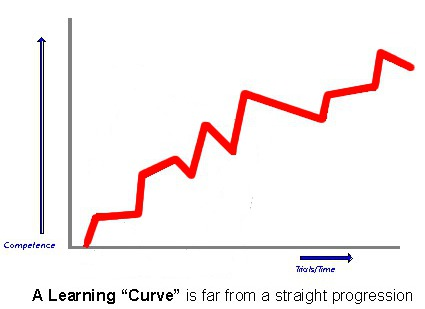
\includegraphics[width=1\textwidth]{images/learning-curve.jpg}

    \column{0.55\textwidth}
      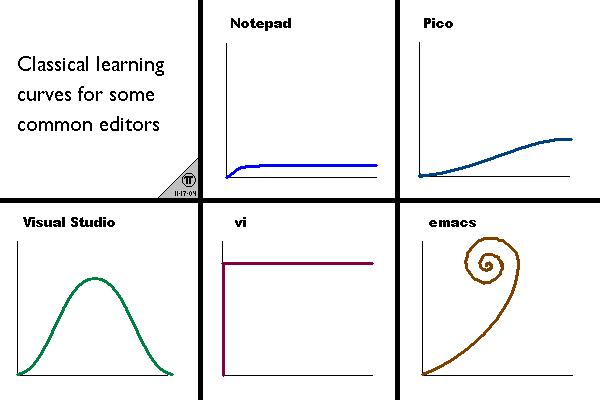
\includegraphics[width=1\textwidth]{images/curves.jpg}
  \end{columns}

  \footnotetext[1]{\tiny \url{http://www.learningandteaching.info/learning/learning_curve.htm} \cite{curve1}}
  \footnotetext[2]{\tiny \url{http://www.terminally-incoherent.com/blog/2006/08/01/text-editor-learning-curves/} \cite{curve2}}
}

\frame{
  \frametitle{Herausforderungen 2}

  ,,We might already be beyond the age of speed, by moving into the age of real-time.''
  - Ivan Illich, Austrian philosopher (1926-2002)

  Weitere Herausforderungen:

  \begin{itemize}
    \item Gruppenverhalten und -Rollen \cite{Huebner:2011}
      % Verschiedene Erwartungen, potentielle Konflikte, unterschiedliche Wahrnehmung (Konstruktivismus)
    \item Konstruktivismus \cite{Watzlawick:1992}
  \end{itemize}
}

\frame{
  \frametitle{Das Unternehmen als Individuum}

  \begin{itemize}
    % \item Möglich, aufgrund langfristiger Erreichung gemeinsamer Ziele
    \item Analogie um Lernprozesse im Unternehmen besser nachvollziehen zu können
    \item Unternehmskultur entspricht der Persönlichkeit
    \item Das unternehmerische Handeln ist das bewusste Tun, wodurch es sich selbst oder seine Umwelt verändert
    \item Die Wissensbasis bestimmt das Handeln
    \item Dessen Konsequenzen initiieren den Lernprozess
    \item Der Lernprozess verändert die Wissensbasis
  \end{itemize}

  \begin{block}{Resultat}
    Bessere Systemanpassung und Problemlösungsfähigkeit
  \end{block}

  % Beispiel
}

\frame{
  \frametitle{Das lernende Unternehmen: in der Vergangenheit}

  \begin{columns}
    \column{0.65\textwidth}
      Beginn der Disziplin:

      \begin{itemize}
        \item 1950-60er Jahre
        \item Passive Rolle des Unternehmens
        \item Ausschließlich ,,Reagieren''
      \end{itemize}

    \column{0.35\textwidth}
      
\includegraphics[width=1\textwidth]{images/buecher.jpg}
  \end{columns}

  ... Abstecher in die Theorien
}

\subsection{Organisationale Lerntheorien}

\frame{
  \frametitle{Cyert und March}

  Cyert und March:

  \begin{itemize}
    \item Vorher: Unternehmen als rationales, über alle notwendigen Informationen verfügendes System
    \item Cyert und March: Unternehmen als adaptives, sich anpassendes rationales System
          % potentiell verschiedene Systemzustände
          % effektiv realisierter Zustand durch Umwelteinflüsse und eigene Ziele gesteuertes Verhalten bestimmt
  \end{itemize}

  Grundlegene Prinzipien:

  \begin{itemize}
    \item Vermeide Unsicherheit
    \item Halte an bewährten Regelsystemen fest
    \item Benutze einfache Regeln
  \end{itemize}
}

\frame{
  \frametitle{Argyris und Schön}

  Argyris und Schön:

  \begin{itemize}
    \item Unternehmerisches Handeln als individuelles durch Rollen geleitetes Handeln
    \item Geäußerte Handlungstheorien VS reale Gebrauchstheorien
    \item Diskrepanzen initiieren Lernprozesse
    \item Drei Lerntypen
      \begin{itemize}
        \item Single-Loop
          % Zielabweichungen werden erkannt und korrigiert
          % Nur Anpassung der Parameter in vorgegebenem Schemata
          % Beispiel: Sinkender Absatz erfordert mehr Werbung und Verkaufsaktivitäten
        \item Double-Loop
          % Lernen durch Bewertung und Entwicklung von Schemata
          % Modifikation und Verbesserung der allgemeinen Regeln, Normen und Ziele
          % Quasi: Ursachenanalyse
          % Beispiel: sinkender Absatz führt zur Überprüfung, ob dies an zu wenig Werbung oder mangelnder Produktqualität liegt
        \item Deutero
          % Lernendes Lernen, höchstes Lernniveau
          % Selbstreflexion der Lernprozesse, mit Wissen aus vergangenen Lernprozessen
      \end{itemize}

      % Wenn Double-Loop oder Deutero Lernen nicht erreicht wird können die Ursachen bspw. in defensivem Verhalten der Miterbeiter liegen
      % und dem Wunsch negative Gefühle zu vermeiden. Probleme werden dann vertuscht und unterdrückt um vor negativen Gefühlen zu schützen.
  \end{itemize}

  Erfordert offene und konstruktive Lern- und Diskussionskultur
}

\frame{
  \frametitle{P. Senge}

  \begin{block}{Unternehmen sind}
    ,,ein Ort, an dem Menschen kontinuierlich entdecken, dass sie ihre Realität
    selbst erschaffen. Und dass sie sie verändern können.''
  \end{block}

  \vspace{0.3cm}

  Sieben Hindernisse:

  \vspace{0.3cm}

  \begin{columns}
    \column{0.6\textwidth}
      \begin{itemize}
        \item Ich bin meine Position
        \item Der Feind da draußen
        \item Angriff ist die beste Verteidigung
        \item Fixierung auf Ereignisse
      \end{itemize}

    \column{0.6\textwidth}
      \begin{itemize}
        \item Gleichnis vom gekochten Fisch
        \item Illusion aus Erfahrung zu lernen
        \item Mythos vom Managementteam
      \end{itemize}
  \end{columns}
}

\frame{
  \frametitle{,,Fünf Disziplinen'' als Lösung}

  \begin{center}
    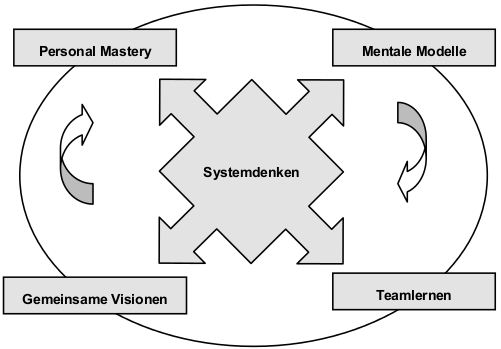
\includegraphics[width=0.8\textwidth]{images/senge.png}
  \end{center}
}

\frame{
  \frametitle{Das lernende Unternehmen: im Jetzt}

  Nur ein lernfähiges Unternehmen kann in einer Wissensgesellschaft erfolgreich
  sein. \cite{Franken:2007}

  \vspace{0.3cm}

  Nonaka und Takeuchi:

  \begin{itemize}
    \item Schaffung neuen Wissens steht über Wissensverarbeitung
    \item Ständige Erneuerung der Denk- und Handlungsmodelle
    \item Lerndimensionen im Unternehmen:
    \begin{itemize}
      \item Epistemologische Dimension: explizites und implizites Wissen
      \item Ontologische Dimension: Individuum und Kollektiv
    \end{itemize}
  \end{itemize}

  Nur Einzelpersonen erzeugen Wissen. Das Unternehmen muss deren Kreativität
  unterstützen, und im Wissensnetz verankern.
}

\frame{
  \frametitle{Nonaka und Takeuchi: die vier Dimensionen}

  \begin{center}
    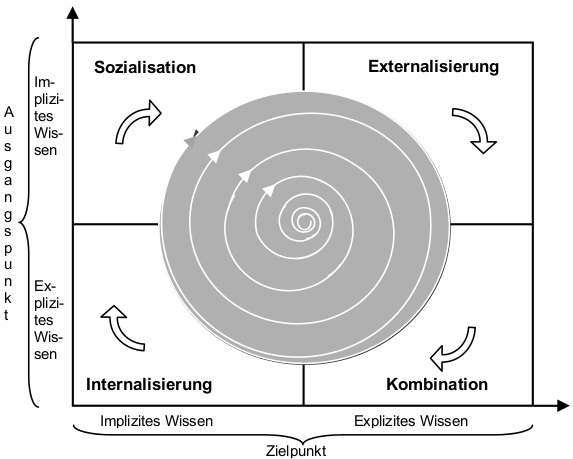
\includegraphics[width=0.8\textwidth]{images/nonaka.png}
  \end{center}

  % Verschiedene Phasen der Wissensgewinnung:
  % - Wissen austauschen
  % - Konzepte schaffen
  % - Konzepte erklären
  % - Einen Archetyp bilden
  % - Wissen übertragen

  % Verschiedene Vorraussetzungen:
  % - Intention
  % - Autonomie
  % - Redundanz
  % - Fluktuation und kreatives Chaos
  % - Notwendige Vielfalt
}

\subsection{Kritik}

\frame{
  \frametitle{Das lernende Unternehmen: in der Zukunft}

  Meine Bewertung: die Theorien gehen nicht weit genug

  \begin{itemize}
    \item Welche Arbeitsbedingungen sind förderlich fürs Lernen
    \item Konstruktivismus \cite{Watzlawick:1992}
    \item Auswirkungen der Lernkultur
    \item Umgang mit Fehlern, Fehlerkultur
    \item Digitales Zeitalter
  \end{itemize}
}

\frame{
  \frametitle{Konnektivismus}

  Konnektivismus:

  \begin{itemize}
    \item Der Mench wird nicht länger als ,,isoliertes'' Wesen betrachtet
    \item Zugriff auf verschiedene Netzwerke möglich
  \end{itemize}
}

\frame{
  \frametitle{Lernkultur}

  \begin{center}
    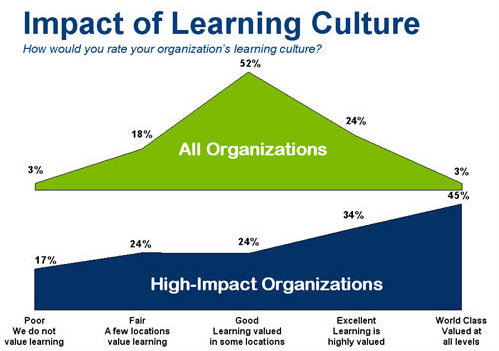
\includegraphics[width=0.8\textwidth]{images/culture.jpg}
  \end{center}

  \footnotetext[1]{\tiny \url{http://joshbersin.com/2008/08/13/the-hilo-80-leaders-in-corporate-learning/} \cite{culture}}
}

\subsection{Zusammenfassung}

\frame{
  \frametitle{Zusammenfassung}
}


